\chapter{Evaluation}

\chapterintro{
  This chapter contains results and discussions on the evaluation of tests run on the proposed solution.
}

\section{Introduction}
We carried out a number of tests which aim to prove the solution be better than currently available, especially in terms of:
\begin{enumerate}
  \item maximum reduction of deployment cost by deploying different stacks comprising a given service on different cloud providers
  \item reduced deployment time
  \item TODO dopisać jeszcze kolejne
\end{enumerate}

\section{Cost of service deployment}
\subsection{Description and preconditions}
The aim of this test case is to test the primary use case of the proposed solution -- deployment of a service with the emphasis of client's \textbf{cost}.
Service specification (\ref{lst:service-spec-test-cost}) forms an input to the application. Its elements are different software stacks that are parts of the whole service. Each cloud provider has its own price for a given software stack which is shown in table \ref{tbl:test-service-deployment-cost}.
This test should show that the platform chooses the best mapping between the stacks and cloud providers so that the client's pays the \textbf{lowest} possible price.

\begin{table}
  \centering
  \begin{tabular}{ | c | c | c | c | }
    \hline                        
    & CP-1 & CP-2 & CP-3 \\
    \hline
    java      & 150 & 120 & 180 \\
    ruby      & 220 & 290 & 250 \\
    postgres  & 320 & 240 & 290 \\
    python    & 200 & 260 & 180 \\
    amqp      & 330 & 390 & 285 \\
    \hline  
  \end{tabular}
  \caption{Price for a stack in the given cloud provider}
  \label{tbl:test-service-deployment-cost}
\end{table}

\subsection{Results}
Table \ref{tbl:test-service-deployment-cost-mapping} shows obtained mapping between stacks and cloud providers. Taking into account this result, figure \ref{ch7:service-deployment-cost} shows comparison of cost the client would have to pay with and without such a mapping.

\begin{table}
  \centering
  \begin{tabular}{ | c | c | c | c | }
    \hline                        
    & CP-1 & CP-2 & CP-3 \\
    \hline
    java      & & x & \\
    ruby      & x & & \\
    postgres  & & x & \\
    python    & & & x \\
    amqp      & & & x \\
    \hline  
  \end{tabular}
  \caption{Chosen cloud providers for the given stack}
  \label{tbl:test-service-deployment-cost-mapping}
\end{table}

\begin{figure}[!ht]
  \begin{center}
    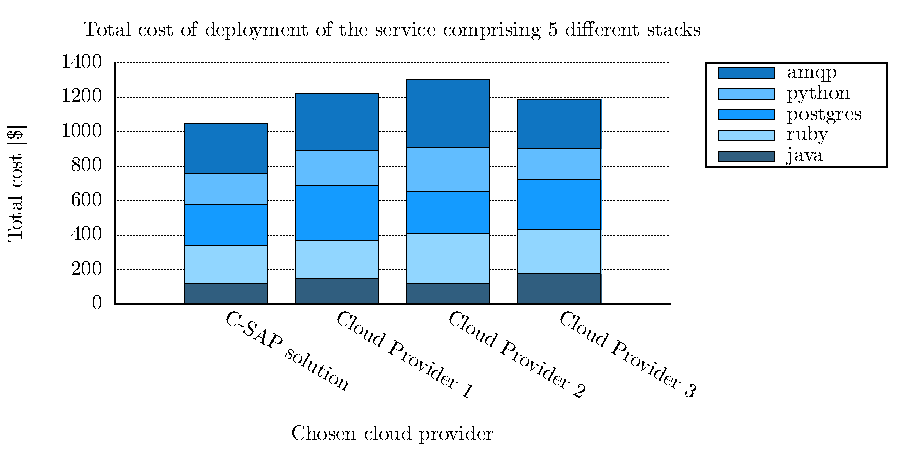
\includegraphics{chapter-7/case-study-service-deployment-reduced-client-costs}
  \end{center}
  \caption{Comparison of the deployment cost when the service is deployed only on a selected cloud provider or a combination of cloud providers selected by Cloud-SAP}
  \label{ch7:service-deployment-cost}
\end{figure}

\section{Deployment time -- solution comparison}
\subsection{Motivation}
In this test we want to compare our solution to one of those available at the market which use \emph{OpenNebula} as an underlying tool for managing resources of a data center and \emph{OpenVZ} as a hypervisor in terms of \textbf{deployment time}, one of the most important factors of products whose main purpose is to scale applications.
\emph{Carina} \cite{Carina} can be considered a perfect match of a solution for such a comparison and tests are ran against it.
\subsection{Description and preconditions}
This test involves the steps of
  \begin{inparaenum}[i)]
    \item instantiating one of the tested product, i.e. Cloud-SAP or Carina,
    \item ordering the deployment of a service whose specification is shown in listing \ref{lst:service-spec-test-deployment-time},
    \item measuring the time needed to set up the environment of the service.
  \end{inparaenum}
Before performing any tests all virtual machines present at the deployment node are removed.
\subsubsection{Service description}
The service comprises a simple java enterprise application, deployed in a master-slave configuration with one VM set as a load balancer and other nodes that serve as workers, which uses Tomcat as a web container.

TODO dodać konfigurację każdej z maszyn wirtualnych
\subsubsection{Hardware configuration}
All virtual machines were deployed on one node which had 3G RAM, AMD Athlon\texttrademark 64 X2 Dual Core Processor with each core of 2000 MHz frequency and a hard drive with a capacity of 160 GB.
\subsection{Results}
Obtained results are shown in table \ref{tbl:test-service-deployment-time} and in figure \ref{ch7:deployment-time-test}.

\begin{table}
  \centering
  \begin{tabular}{ c  c  c }
    \hline
    & \multicolumn{2}{c}{Solution} \\
    \cline{2-3}
    Instance no & Cloud-SAP & Carina \\
    \hline
    2 & 103.9s & x \\
    3 & 166.3s & x \\
    4 & 225.5s & x \\
    5 & 288.3s & x \\
    \hline
  \end{tabular}
  \caption{Average deployment time for the service with the various number of VMs used for the whole environment}
  \label{tbl:test-service-deployment-time}
\end{table}

\begin{figure}[!ht]
  \begin{center}
    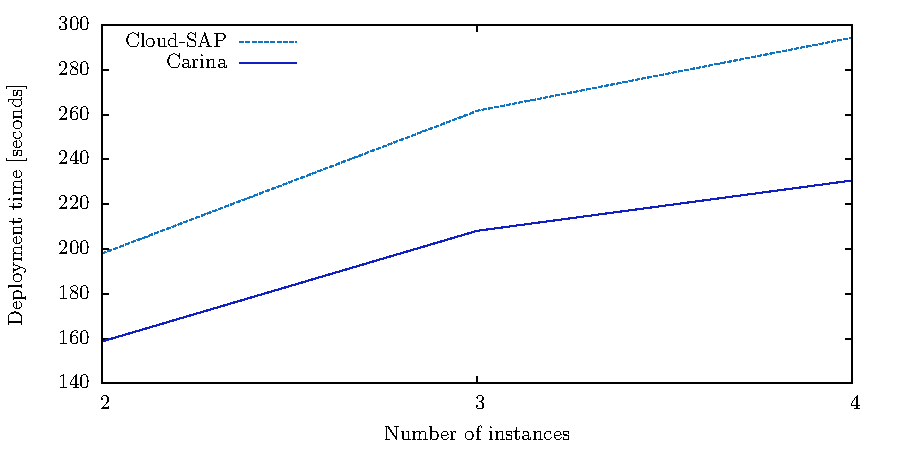
\includegraphics{chapter-7/deployment-time-test}
  \end{center}
  \caption{Average deployment time for two competing products when the variable is the number of instances of VMs}
  \label{ch7:deployment-time-test}
\end{figure}

\section{Deployment time -- hypervisor comparison}

\section{Auto-scaling}
